\input{commun/presentations.tex}

\title[Séance 9 - Espaces aériens \& Sécurité]{Séance 9 \\ Espaces aériens \& Sécurité}

\begin{document}
 \begin{frame}
 \titlepage
 \end{frame}
 
 \begin{frame}{La cartographie et la navigation}
 	\question{A votre avis, quelles sont les règles de priorité entre catégories d'aéronef, \pause pour un dépassement, \pause pour un croisement ?}
 
 \end{frame}
 
 \begin{frame}
 \tableofcontents
 \end{frame}
 
 \section{Règles de l'air}
 	\subsection{Priorités}
	\begin{frame}{Priorité - entre aéronefs}
	\begin{columns}
		\begin{column}{0.5\textwidth}
		\begin{figure}[H]
			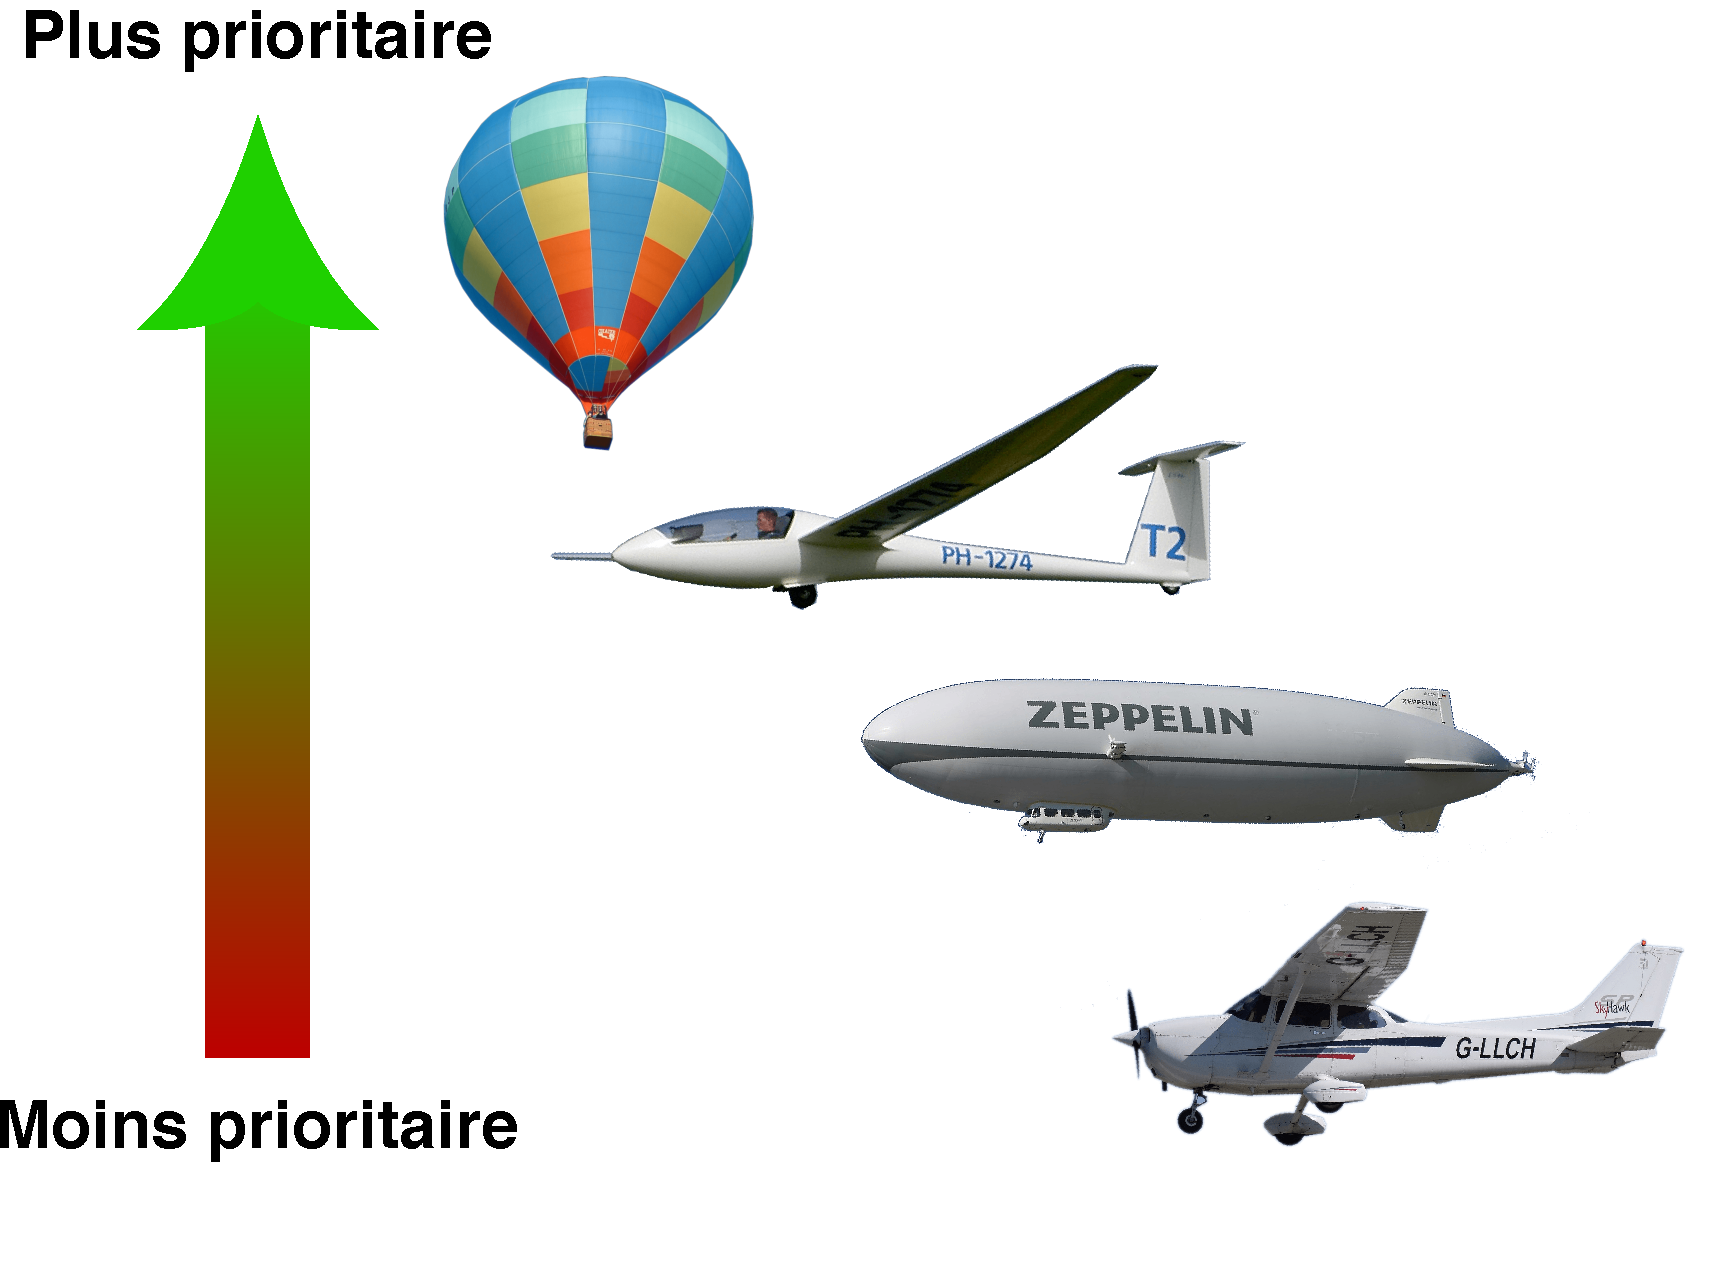
\includegraphics[width=1\linewidth]{02-Navigation/img/priorite_entreAeronefs.pdf}
			\legende{Priorités entre catégories d'aéronefs}{img:priorite_entreAeronefs}
		\end{figure}	
		\end{column}
		\begin{column}{0.5\textwidth}
			\begin{itemize}
				\item Les aéronefs non motorisés sont prioritaires sur les motorisés
				\item Un aéronef qui en remorque un autre est prioritaire sur les autres
				\item Un aéronef en vol est prioritaire sur un aéronef au sol
			\end{itemize}
		\end{column}
	\end{columns}
	\end{frame} 	
 	
	\begin{frame}{Priorité - dépassement}
	\begin{columns}
		\begin{column}{0.5\textwidth}
		\begin{figure}[H]
			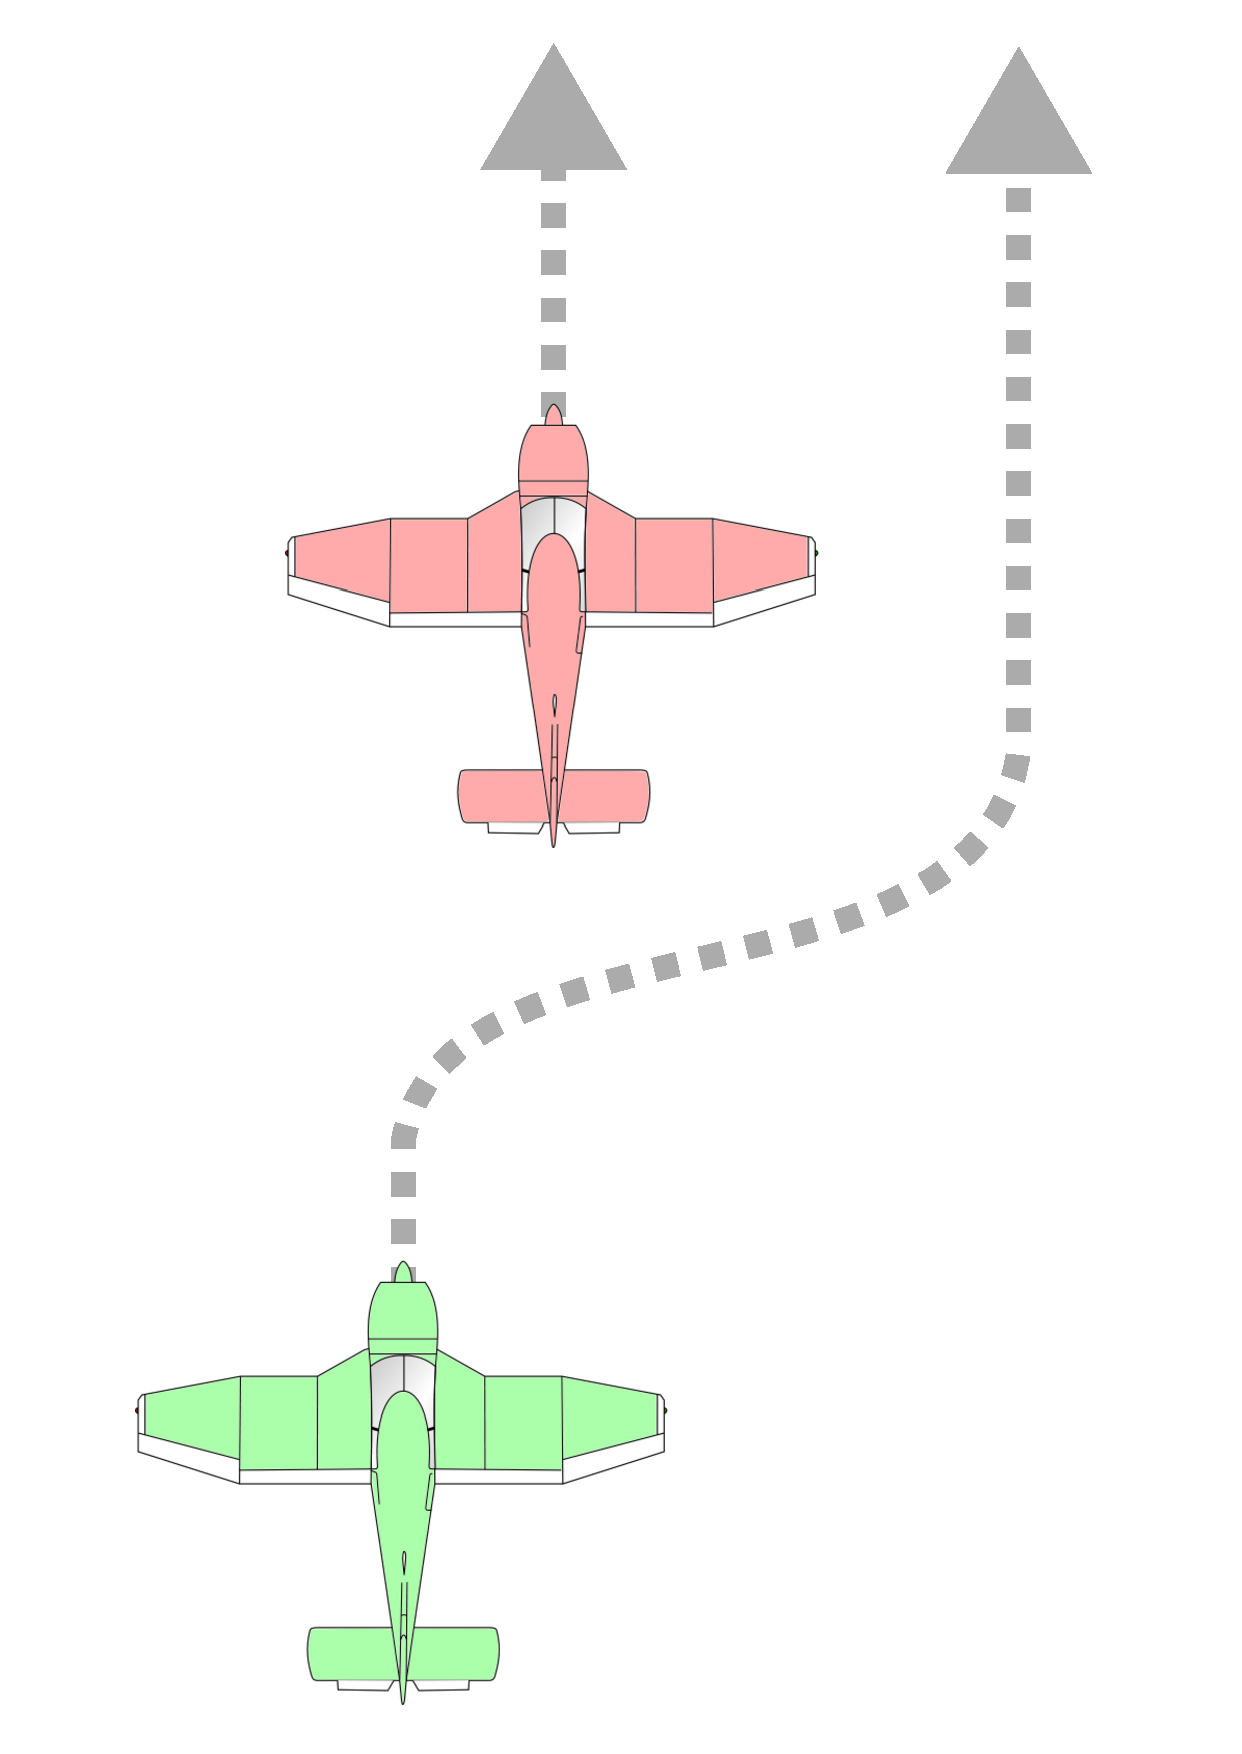
\includegraphics[width=0.5\linewidth]{02-Navigation/img/priorite_plusRapide.pdf}
			\legende{Dépassement d'un aéronef moins rapide}{img:priorite_plusRapide}
		\end{figure}	
		\end{column}
		\begin{column}{0.5\textwidth}
			\begin{itemize}
				\item Le dépassement d'un aéronef moins rapide se fait par la droite
			\end{itemize}
		\end{column}
	\end{columns}
	\end{frame}
	
	\begin{frame}{Priorité - route convergente}
	\begin{columns}
		\begin{column}{0.5\textwidth}
		\begin{figure}[H]
			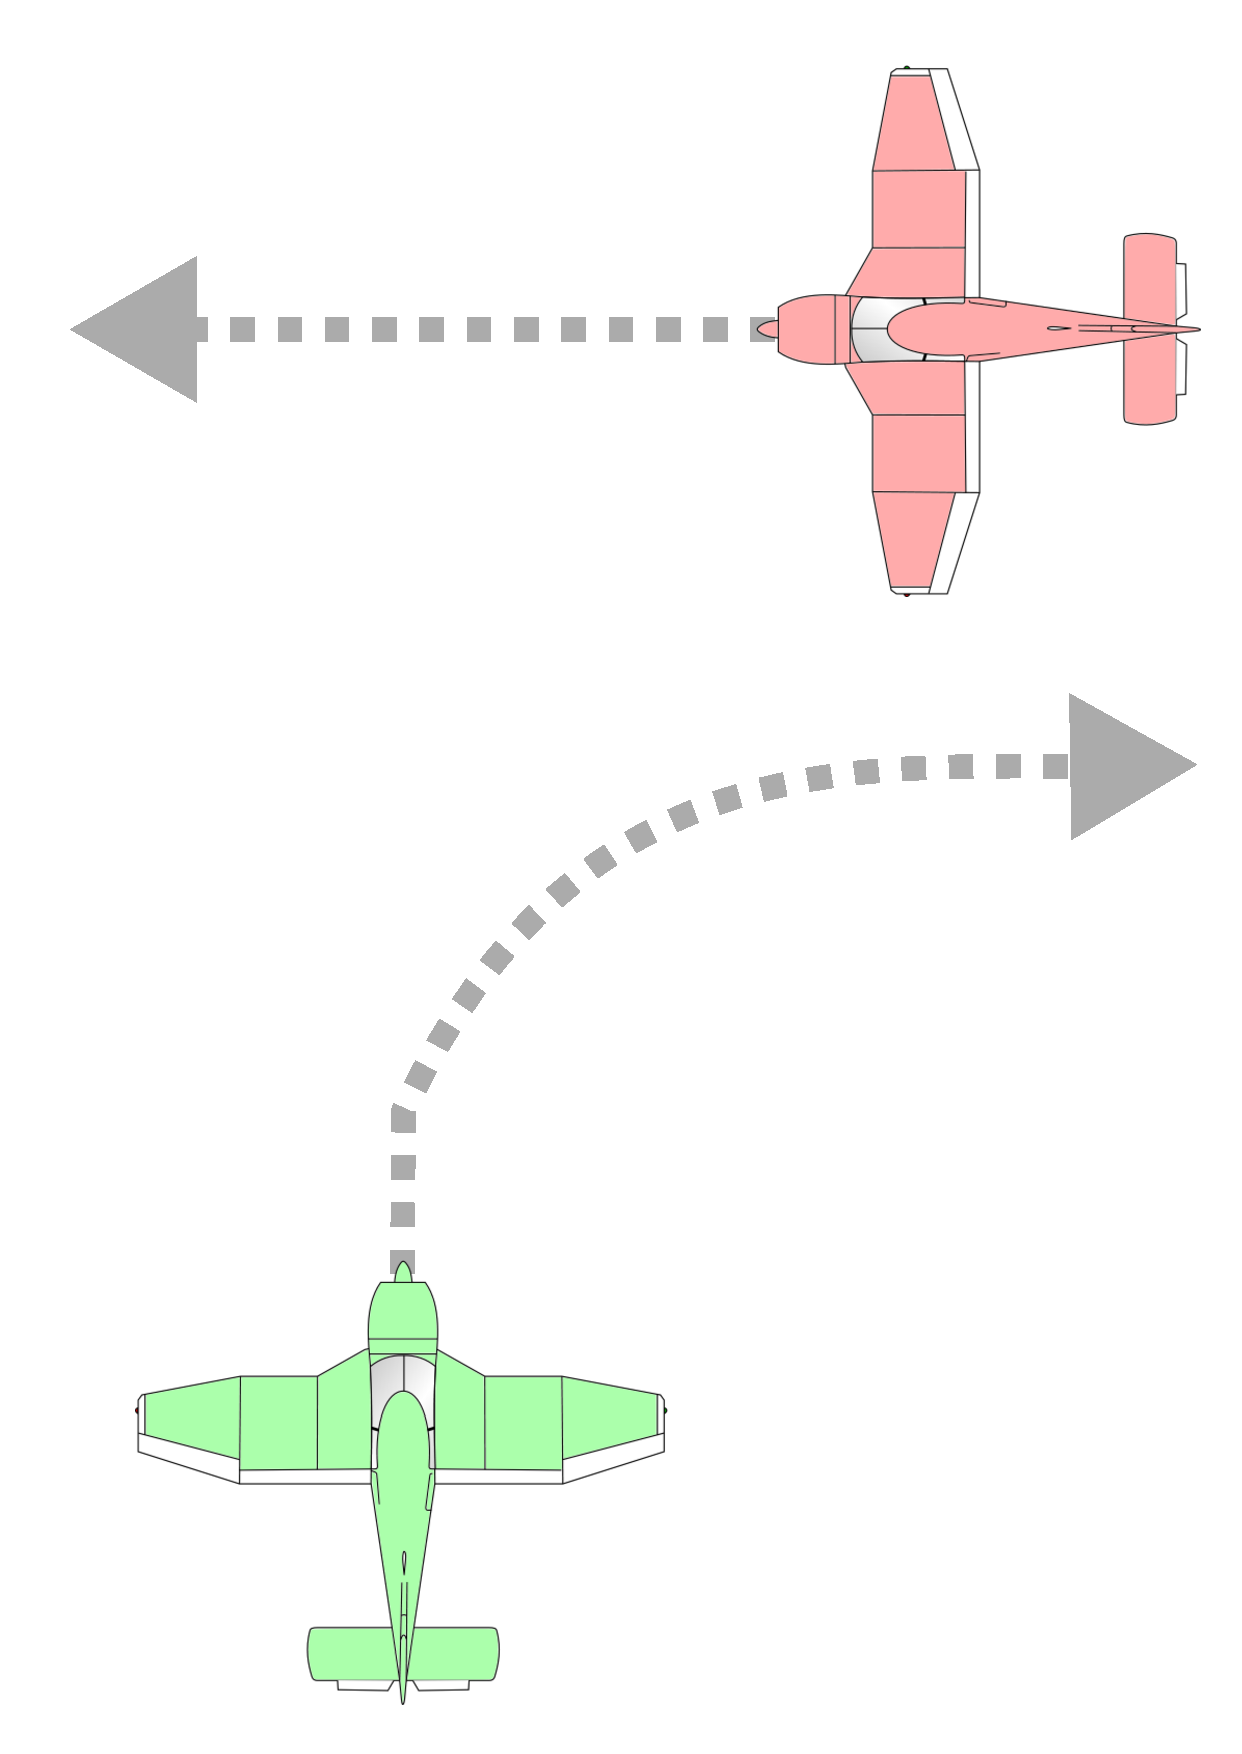
\includegraphics[width=0.65\linewidth]{02-Navigation/img/priorite_convergeant.pdf}
			\legende{Aéronefs avec route convergente}{img:priorite_convergeant}
		\end{figure}	
		\end{column}
		\begin{column}{0.5\textwidth}
			\begin{itemize}
				\item Lorsqu'un aéronef voit un aéronef avec une route convergente à sa droite, il lui cède la priorité
			\end{itemize}
		\end{column}
	\end{columns}
	\end{frame}
	
	\begin{frame}{Priorité - face à face}
	\begin{columns}
		\begin{column}{0.5\textwidth}
		\begin{figure}[H]
			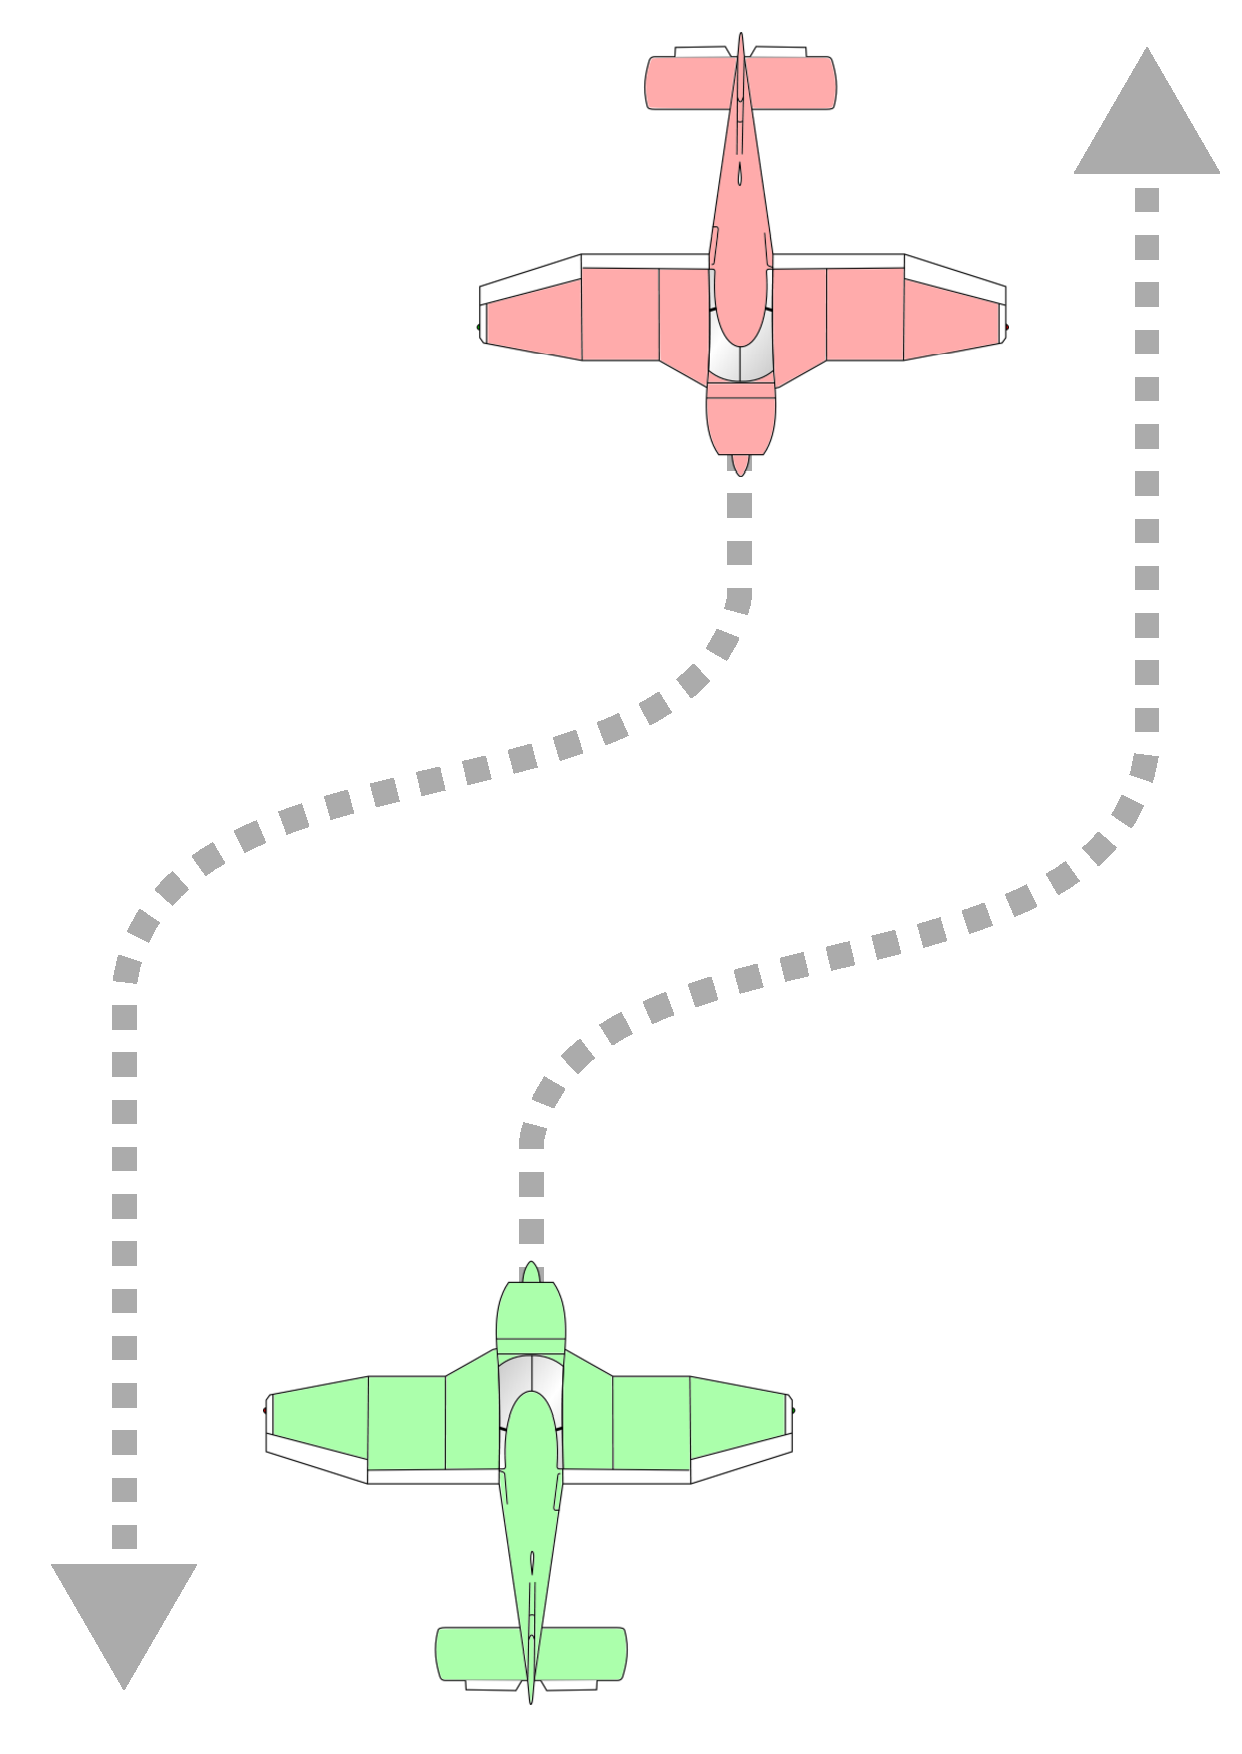
\includegraphics[width=0.65\linewidth]{02-Navigation/img/priorite_faceFace.pdf}
			\legende{Aéronef sur route opposées}{img:priorite_faceFace}
		\end{figure}	
		\end{column}
		\begin{column}{0.5\textwidth}
			\begin{itemize}
				\item Lorsque 2 aéronefs sont face à face, chaque aéronef doit virer à droite
			\end{itemize}
		\end{column}
	\end{columns}
	\end{frame}

	
	 \subsection{Les espaces aériens}
	\begin{frame}{Les espaces aériens}
		L'espace aérien est divisé en différentes zones. Chaque type de zone impose des contraintes aux aéronefs qui veulent y pénétrer, en contrepartie d'un niveau de service.
		
		L'espace aérien est divisé en 7 classes nommées par des lettres, de A à G. 
		
		Il existe également des zones dangereuses, restreintes ou interdites.
	\end{frame}	 
 
 \begin{frame}{Classe A}
 \begin{columns}
		\begin{column}{0.7\textwidth}
 			\begin{figure}[H]
			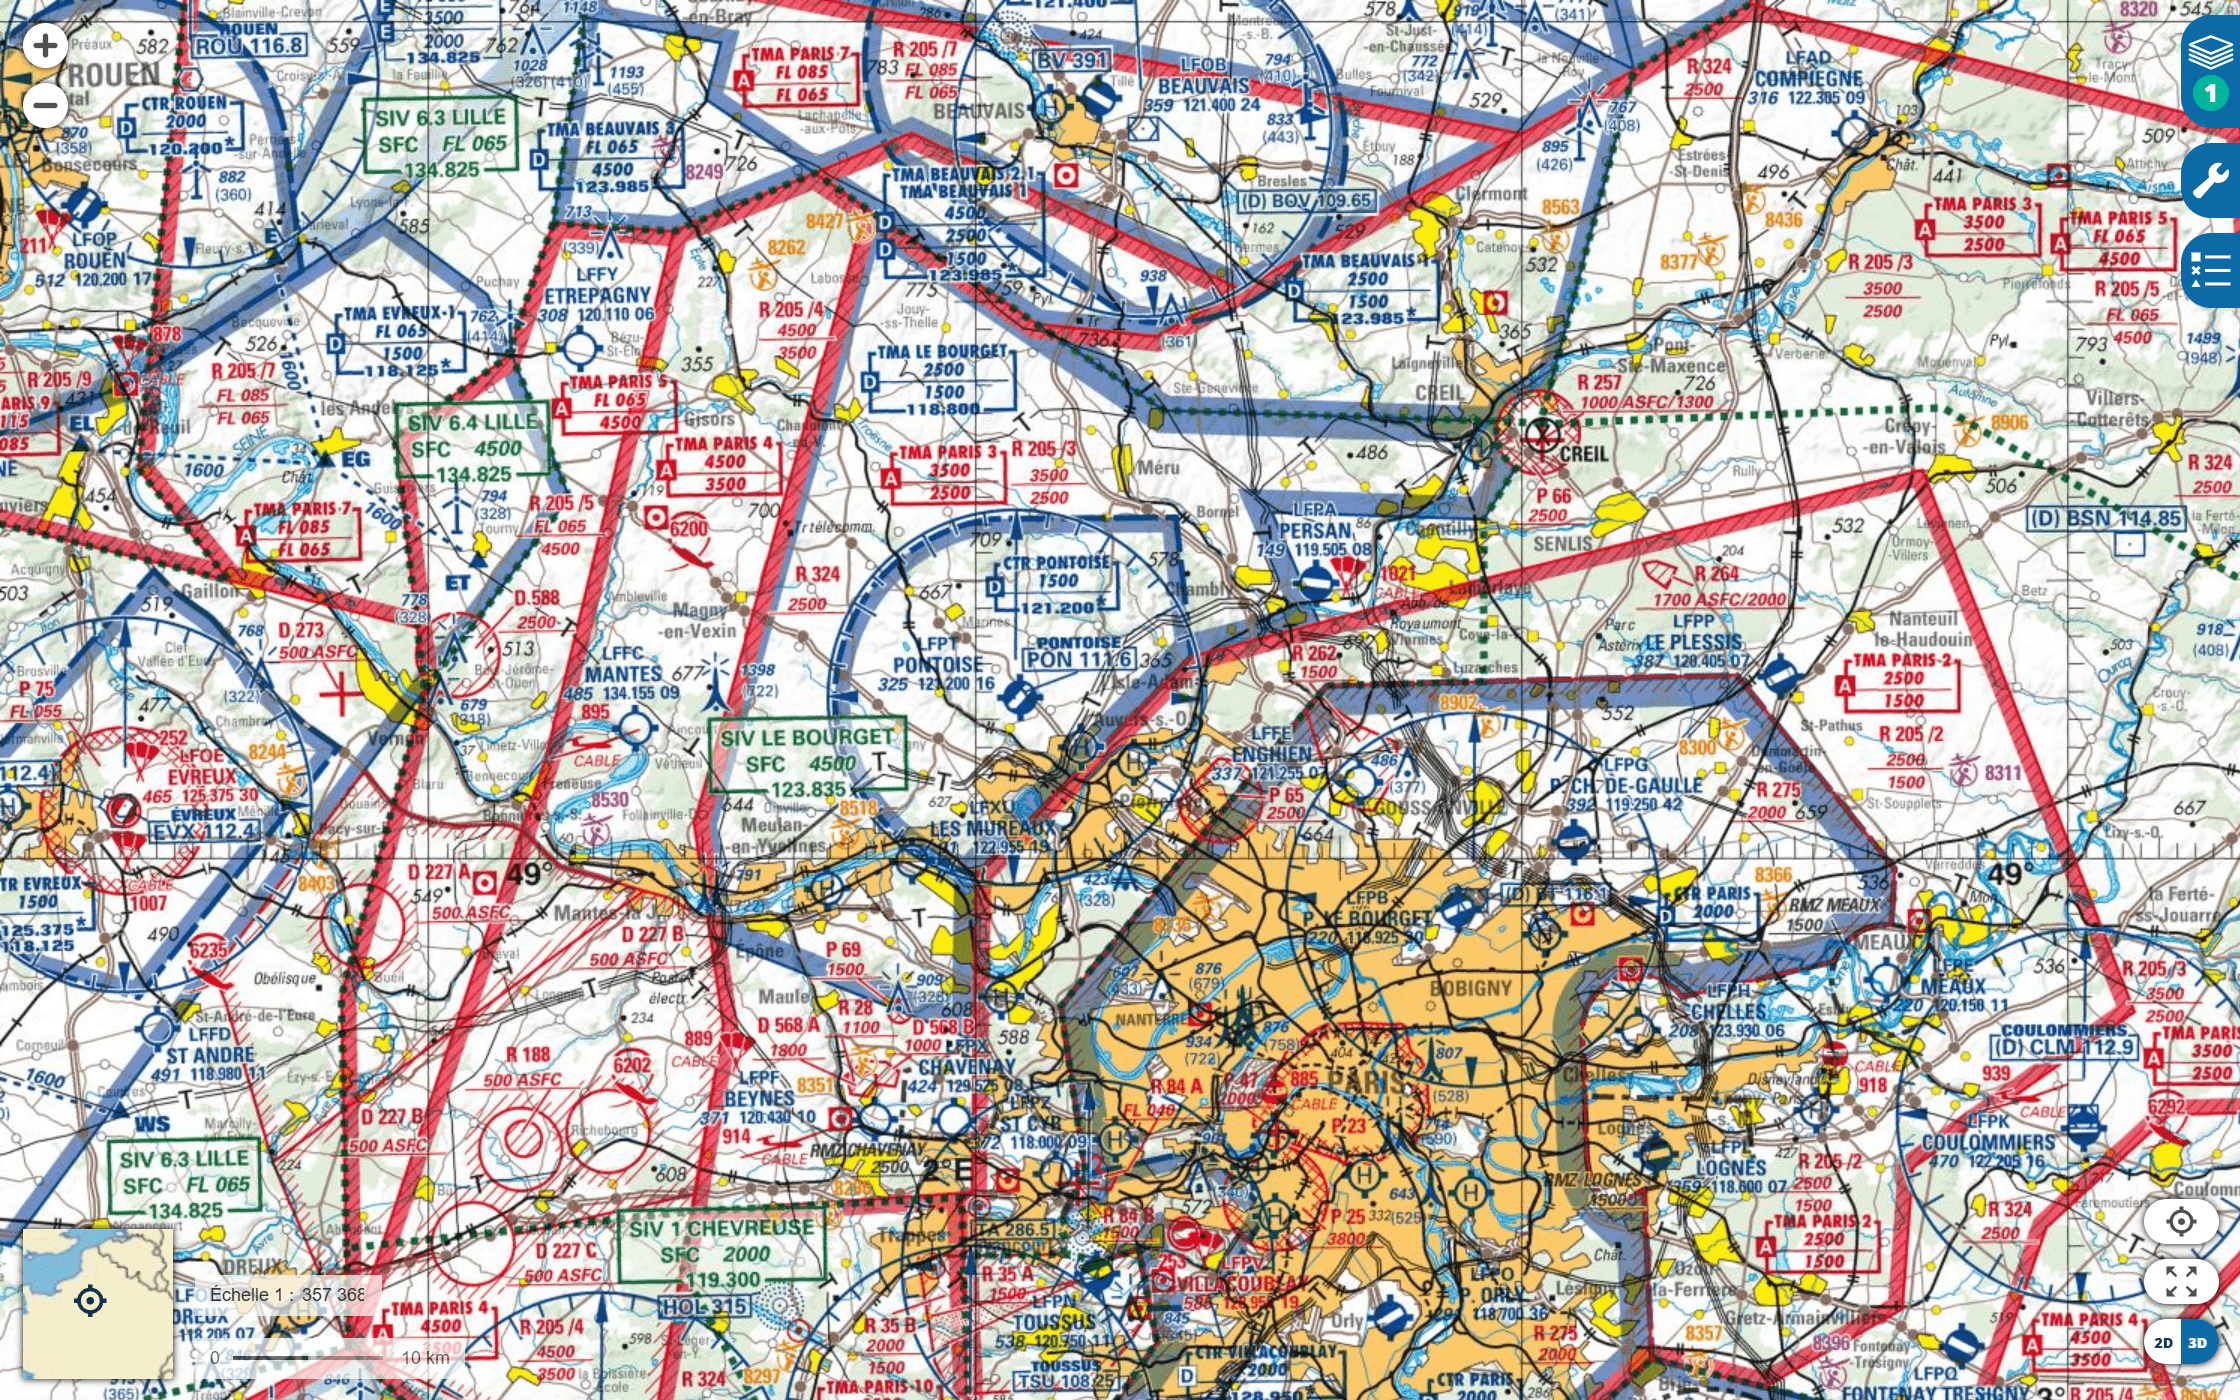
\includegraphics[width=1\linewidth]{Annexes/img/ignOaciParis.png}
			\legende{Extrait de carte de navigation - région parisienne}{img:ignOaciParis}
			\end{figure}	
		\end{column}
		\begin{column}{0.3\textwidth}
		\begin{itemize}
		\item Entrée soumise à \textit{clearance} (autorisation du contrôleur)		
		
		\item Espace interdit aux vols VFR
		
		\item En France : utilisé uniquement en région parisienne
		\end{itemize}
		\end{column}
	\end{columns}
 \end{frame}
 
 \begin{frame}{Classe C et D}
 \begin{columns}
		\begin{column}{0.6\textwidth}
 			\begin{figure}[H]
			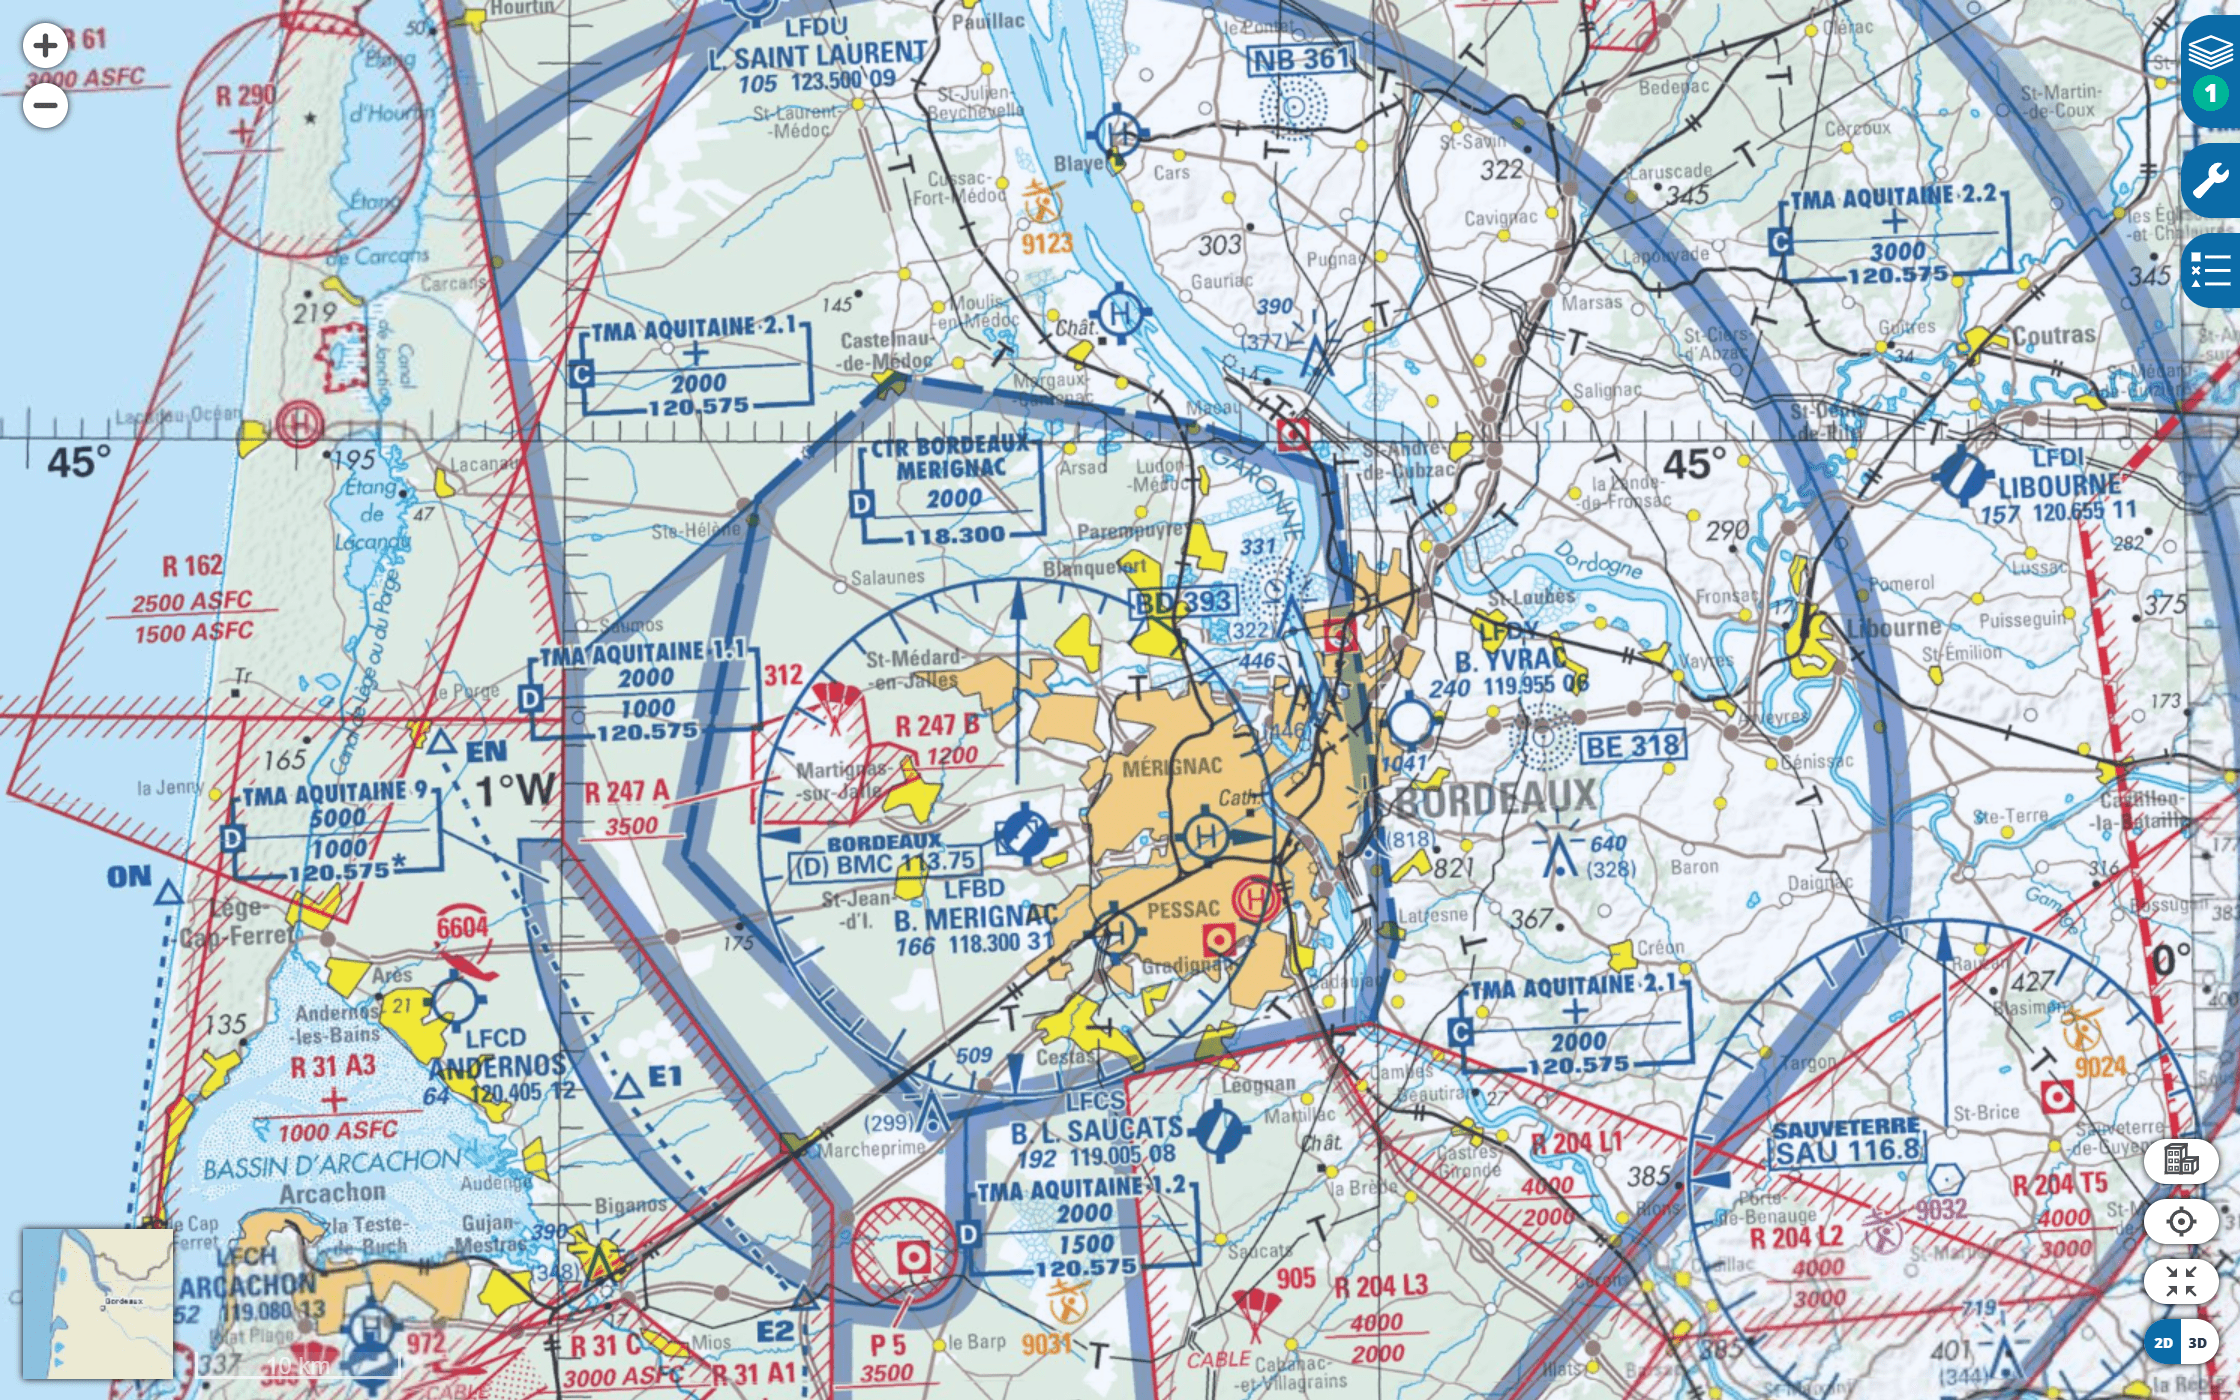
\includegraphics[width=1\linewidth]{Annexes/img/ignOaciBordeaux.png}
			\legende{Extrait de carte de navigation - région de Bordeaux}{img:ignOaciBordeaux}
			\end{figure}	
		\end{column}
		\begin{column}{0.4\textwidth}
		\begin{itemize}
		\item Entrée soumise à \textit{clearance}
		
		\item Autorisé au VFR et aux IFR
		
		\item En France : utilisé pour les zones d'approche des aéroports
		
		\item C : le contrôleur assure la séparation entre IFR et entre IFR et VFR
		
		\item D : le contrôleur assure la séparation entre IFR
		\end{itemize}
		\end{column}
	\end{columns}
 \end{frame}
 
 \begin{frame}{Classe G}
 \begin{columns}
		\begin{column}{0.6\textwidth}
 			\begin{figure}[H]
			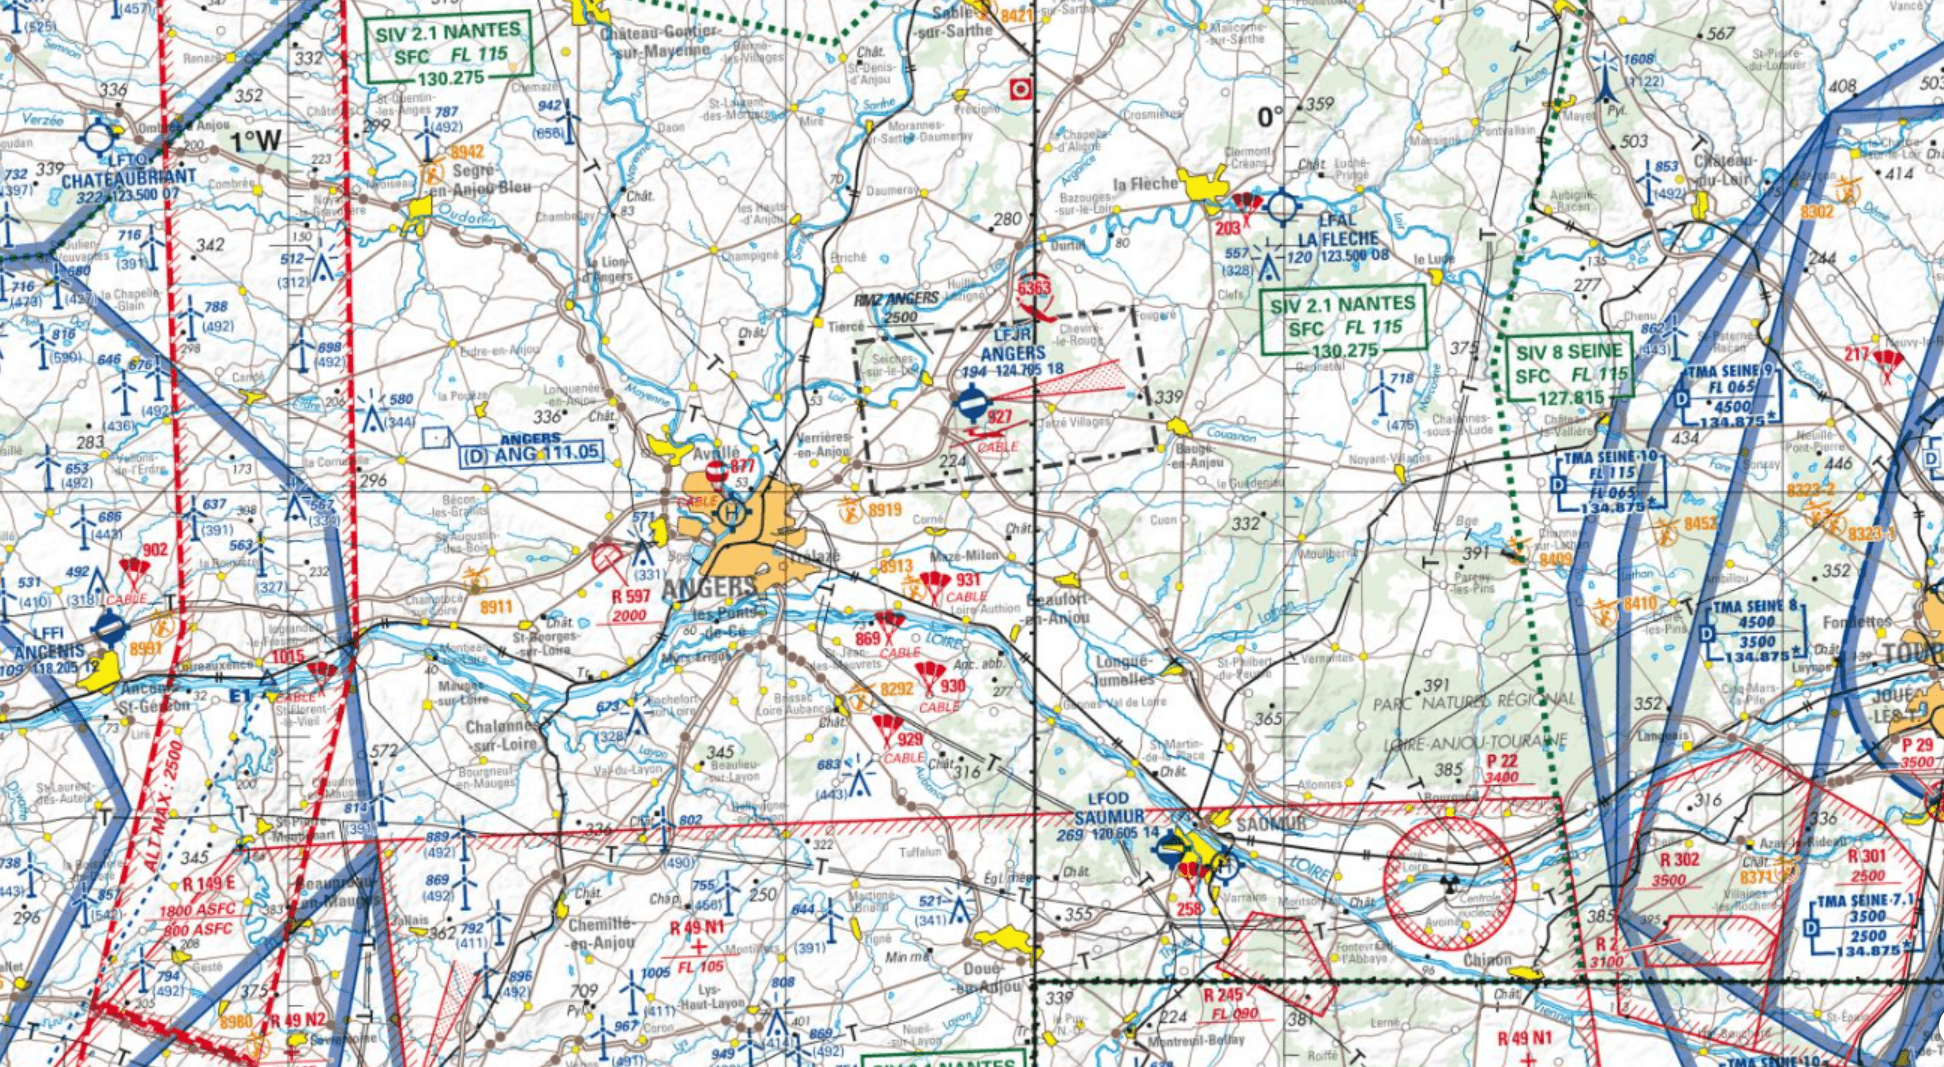
\includegraphics[width=1\linewidth]{Annexes/img/ignOaciAngers.png}
			\legende{Extrait de carte de navigation - région d'Angers}{img:ignOaciAngers}
			\end{figure}	
		\end{column}
		\begin{column}{0.4\textwidth}
		\begin{itemize}
		\item L'espace aérien "par défaut" est de classe G
		\item C'est un espace aérien non contrôlé : tous les vols (IFR/VFR) doivent assurer eux même l'anti-abordage
		\end{itemize}
		\end{column}
	\end{columns}
 \end{frame}
 
 \begin{frame}{Les zones à statut particulier}
		En plus des classes d'espace aérien, il existe des zones à statut particulier : les zones interdites, restreintes, dangereuses
	\end{frame}	
 
 \begin{frame}{Zones P - Prohibée}
 \begin{columns}
		\begin{column}{0.5\textwidth}
 			\begin{figure}[H]
			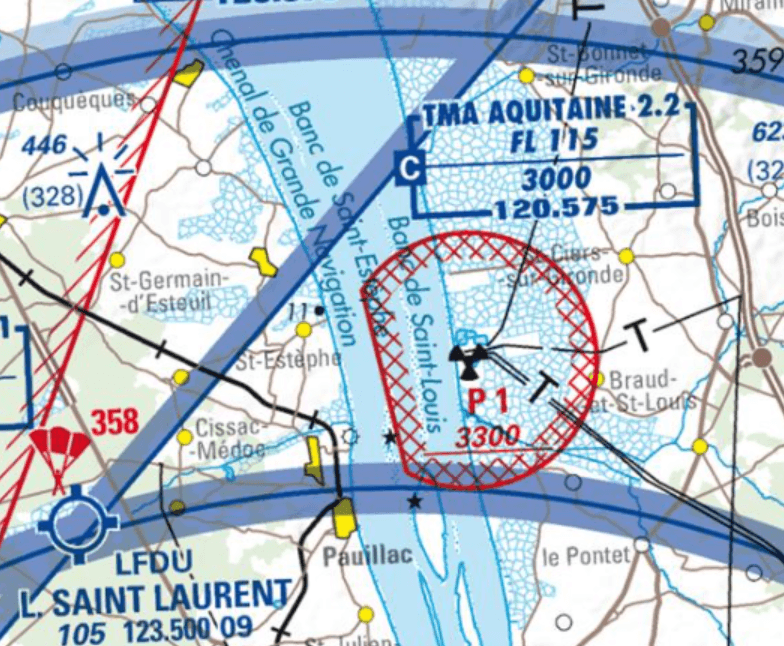
\includegraphics[width=\linewidth]{02-Navigation/img/IGN_OACI_P1.png}
	\legende{La zone interdite P1}{img:ignOaci}
			\end{figure}	
		\end{column}
		\begin{column}{0.5\textwidth}
		\begin{itemize}
		\item Zone dans laquelle il est interdit de rentrer
		\item en France, autour des centrales nucléaires, Paris, les bases militaires importantes...
		\end{itemize}
		\end{column}
	\end{columns}
 \end{frame}
 
 \begin{frame}{Zones D - Dangereuse}
 \begin{columns}
		\begin{column}{0.5\textwidth}
 			\begin{figure}[H]
			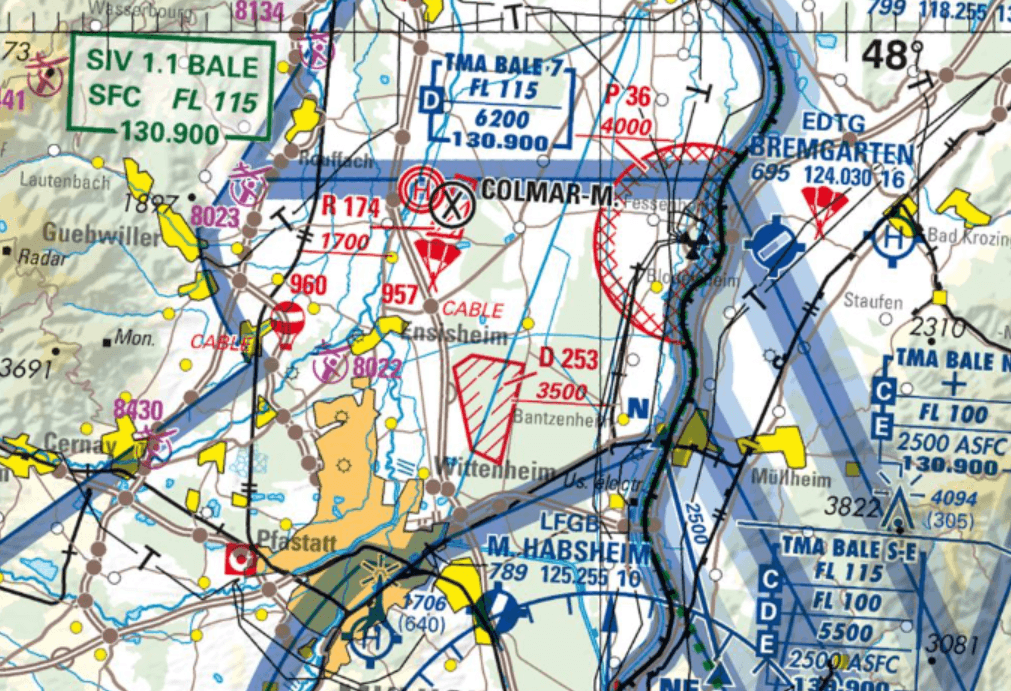
\includegraphics[width=\linewidth]{02-Navigation/img/IGN_OACI_D253.png}
	\legende{La zone dangereuse D253}{img:ignOaci}
			\end{figure}	
		\end{column}
		\begin{column}{0.5\textwidth}
		\begin{itemize}
		\item Zone dans laquelle il est dangereux de rentrer
		\item utilisé pour protéger des champs de tir sol/air par exemple
		\end{itemize}
		\end{column}
	\end{columns}
	
	\alerte{Ne pas confondre avec les espaces aérien de classe D !}
 \end{frame}
 
 
 \begin{frame}{Zones R - Restreinte}
 \begin{columns}
		\begin{column}{0.5\textwidth}
 			\begin{figure}[H]
			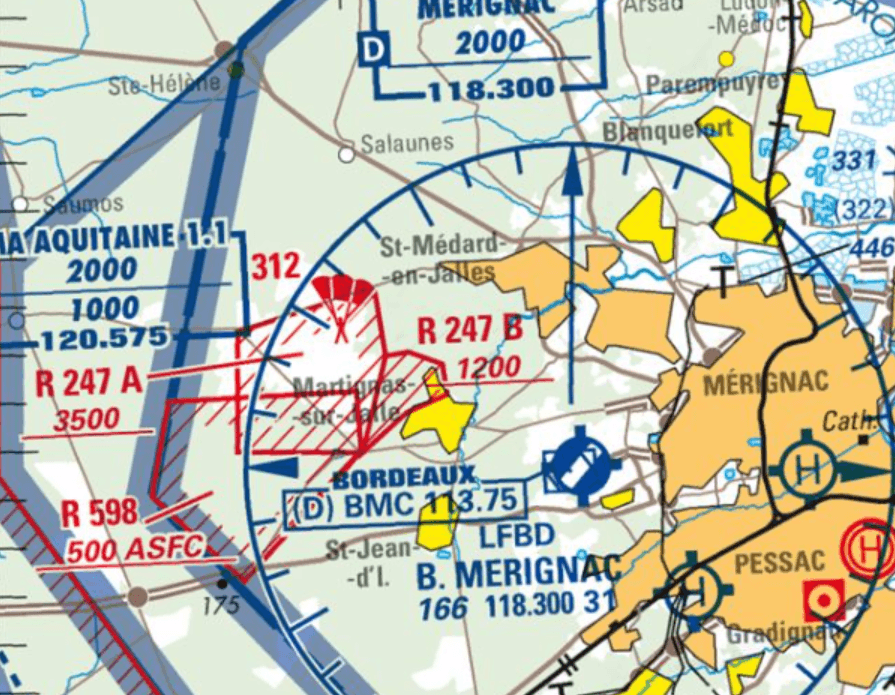
\includegraphics[width=\linewidth]{02-Navigation/img/IGN_OACI_R247_R_598.png}
	\legende{La zone restreinte R257A/B et R598}{img:ignOaci}
			\end{figure}	
		\end{column}
		\begin{column}{0.5\textwidth}
		\begin{itemize}
		\item Zone restreinte à certains usagers
		\end{itemize}
		\end{column}
	\end{columns}
 \end{frame}
 
 
 \section{Communication et sécurité}
 	\subsection{Communications}
 	\begin{frame}{Usage de la radio}
 		La radio est utilisée pour communiquer entre aéronefs (auto-information) ou entre aéronefs et contrôle au sol. La bande aéronautique s'étend sur la bande VHF entre 108 et 137 MHz.
 		
 		Fréquence de détresse : 121.5 MHz
 		
 		
 		\begin{figure}[H]
			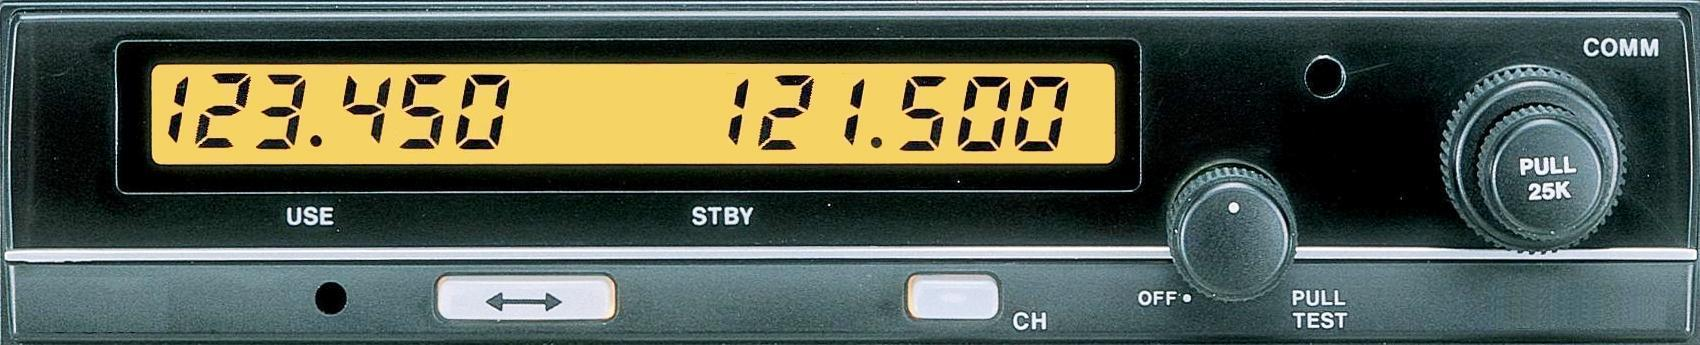
\includegraphics[width=\linewidth]{02-Navigation/img/radioAeronautique.jpg}
	\legende{Poste radio aéronautique}{img:radioAeronautique}
			\end{figure}	
 	
 	\end{frame}
 		
 	\begin{frame}{Alphabet radio international}
 	\centering
 	\begin{tabular}{|c|c||c|c||c|c|}
		\hline
			A & Alpha & 				J & Juliett &			S & Sierra \\
		\hline
			B & Bravo & 				K & Kilo &				T & Tango \\
		\hline
			C & Charlie & 			L & Lima &				U & Uniform \\
		\hline
			D & Delta & 				M & Mike &				V & Victor \\
		\hline
			E & Echo & 				N & November &			W & Whiskey \\
		\hline
			F & Fox-trot & 			O & Oscar &				X & X-Ray \\
		\hline
			G & Golf & 				P & Papa &				Y & Yankee \\
		\hline
			H & Hotel & 				Q & Quebec &				Z & Zoulou \\
		\hline
			I & India & 				R & Romeo &				 & 		\\
		\hline
	\end{tabular}
 	\end{frame}
 		
 		\begin{frame}{Transpondeur}
 		Le transpondeur rend l'avion identifiable par le contrôleur aérien. Il répond aux interrogation des radars secondaires.
 	
 	Le transpondeur peut envoyer des informations : code saisi par le pilote, altitude de l'aéronef, immatriculation...
 		
 		\begin{figure}[H]
			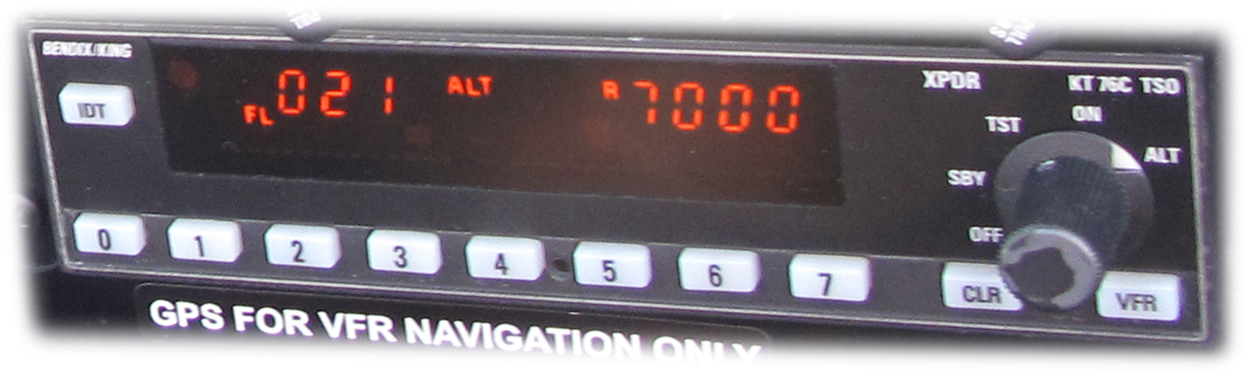
\includegraphics[width=\linewidth]{02-Navigation/img/transpondeur.jpg}
	\legende{Un transpondeur}{img:transpondeur}
			\end{figure}	
 	\end{frame}	
 	
 	\begin{frame}{Transpondeur}		
 		\begin{figure}[H]
			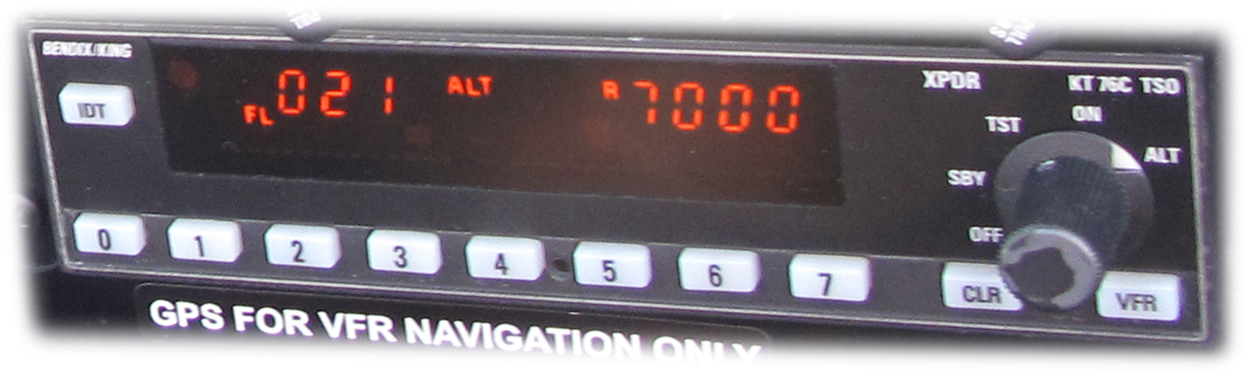
\includegraphics[width=\linewidth]{02-Navigation/img/transpondeur.jpg}
	\legende{Un transpondeur}{img:transpondeur}
			\end{figure}	
 		
 		Des codes à connaitre :
 		\begin{itemize}
 			\item 7000 : code par défaut pour les vols VFR
 			\item 7500 : détournement
 			\item 7600 : panne radio
 			\item 7700 : détresse
 		\end{itemize}
 	\end{frame}	
 
 \subsection{Sécurité}
 \begin{frame}{Sécurité}
 En aéronautique, la plupart des accidents ont des causes humaines (par opposition aux causes météo ou mécaniques par exemple). Les erreurs de pilotage sont à la source d'environ la moitié des accidents.
 
 Pour réduire l'accidentologie, les qualités requises pour un pilote sont une bonne connaissance de soi, de ses limites et de sa machine. 
 
 \end{frame}
 
 \begin{frame}{Sécurité}
	Un accident résulte généralement d'un enchainement de plusieurs erreurs ou défaillances.
	
	Le rattrapage d'une seule des erreurs dans chaine d'erreur évite l'accident.
 
 \begin{figure}[H]
			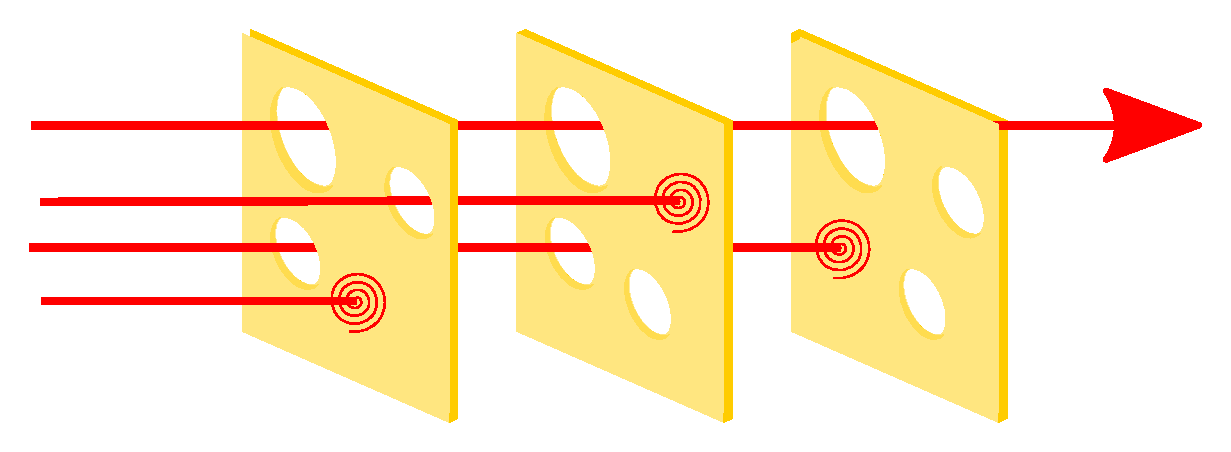
\includegraphics[width=\linewidth]{02-Navigation/img/SwissCheeseModel.pdf}
	\legende{Plaques de Reason ou modèle du fromage suisse}{img:SwissCheeseModel}
			\end{figure}	
 
 \end{frame}
	
\appendix 
\section{QCM}
\qmcBia{Navigation, réglementation, sécurité des vols}
{1}{Pour la sécurité des vols, la qualité qu'il faut avoir en priorité est :}
{une bonne connaissance de soi, de ses limites et de sa machine}
{une grande habileté de pilotage}
{un grand nombre d'heures de pilotage}
{une bonne connaissance de la réglementation} 
{}


\qmcBia{Navigation, réglementation, sécurité des vols}
{1}{Sur une fréquence radio un aéronef immatriculé F-GTAX s'identifie : }
{Fox-Trot-Golf-Tango-Alpha-X-Ray}
{Fox-Golf-Tango-Alpha-Xilo}
{French-Golf-Tango-Alpha-X-Ray}
{Fox-Trot-Golf-Tango-Alpha-Xilo} 
{} 

\qmcBia{Navigation, réglementation, sécurité des vols}
{3}{Sur un aérodrome non contrôlé, l'éventuelle fréquence sur laquelle les pilotes peuvent échanger de l'information est nommée : }
{fréquence d'alerte}
{fréquence de courtoisie}
{fréquence d'auto-information}
{fréquence de détresse} 
{} 

\qmcBia{Navigation, réglementation, sécurité des vols}
{2}{Un aéronef doit dépasser un autre aéronef par : }
{la gauche et il n'est pas prioritaire}
{la droite et il n'est pas prioritaire}
{la droite et il est prioritaire}
{la gauche et il est prioritaire} 
{} 

\qmcBia{Navigation, réglementation, sécurité des vols}
{4}{Un espace de classe G est :}
{contrôlé}
{interdit au VFR}
{autorisé en VFR spécial} 
{non contrôlé}
{} 

\qmcBia{Navigation, réglementation, sécurité des vols}
{1}{Le code standard d'un transpondeur en VFR en l'absence d'instruction du contrôle est : }
{le 7000}
{le 7700}
{le 7600}
{le 7500} 
{} 
 
\input{commun/beamerSlidesBiblio.tex} 
 
\end{document}
